% Charlotte Geiger - Manuel Lippert - Leonard Schatt
% Physikalisches Praktikum

% 3.Kapitel  Protokoll

% Variables
\def\skalierung{0.65}

\chapter{Messprotokoll}
\label{chap:protokoll}

Das Messprotokoll wurde am Versuchstag handschriftlich erstellt und hier als
PDF-Datei eingefügt. 

\section*{Zusatz}
Im Protokoll selbst ist uns dabei ein Fehler unterlaufen, wodurch die Bilder selbst nicht richtig zugeordnet werden können, dafür fügen wir die Bilder mit der korrekten Zuordnung und zur besseren Übersicht am Ende des Protokolls an. Weiterhin werden die verwendeten Schaltungen und Widerstände des Versuchs zusätzlich anfügen.

% Einbindung des Protokolls als pdf (mit Seitenzahl etc.)
% Erste Seite mit Überschrift
%\includepdf[pages = 1, landscape = false, nup = 1x1, scale = \skalierung , pagecommand={\thispagestyle{empty}\chapter{Protokoll}}]
%            {03-Protokoll/Protokoll.pdf}
% Restliche Seiten richtig skaliert
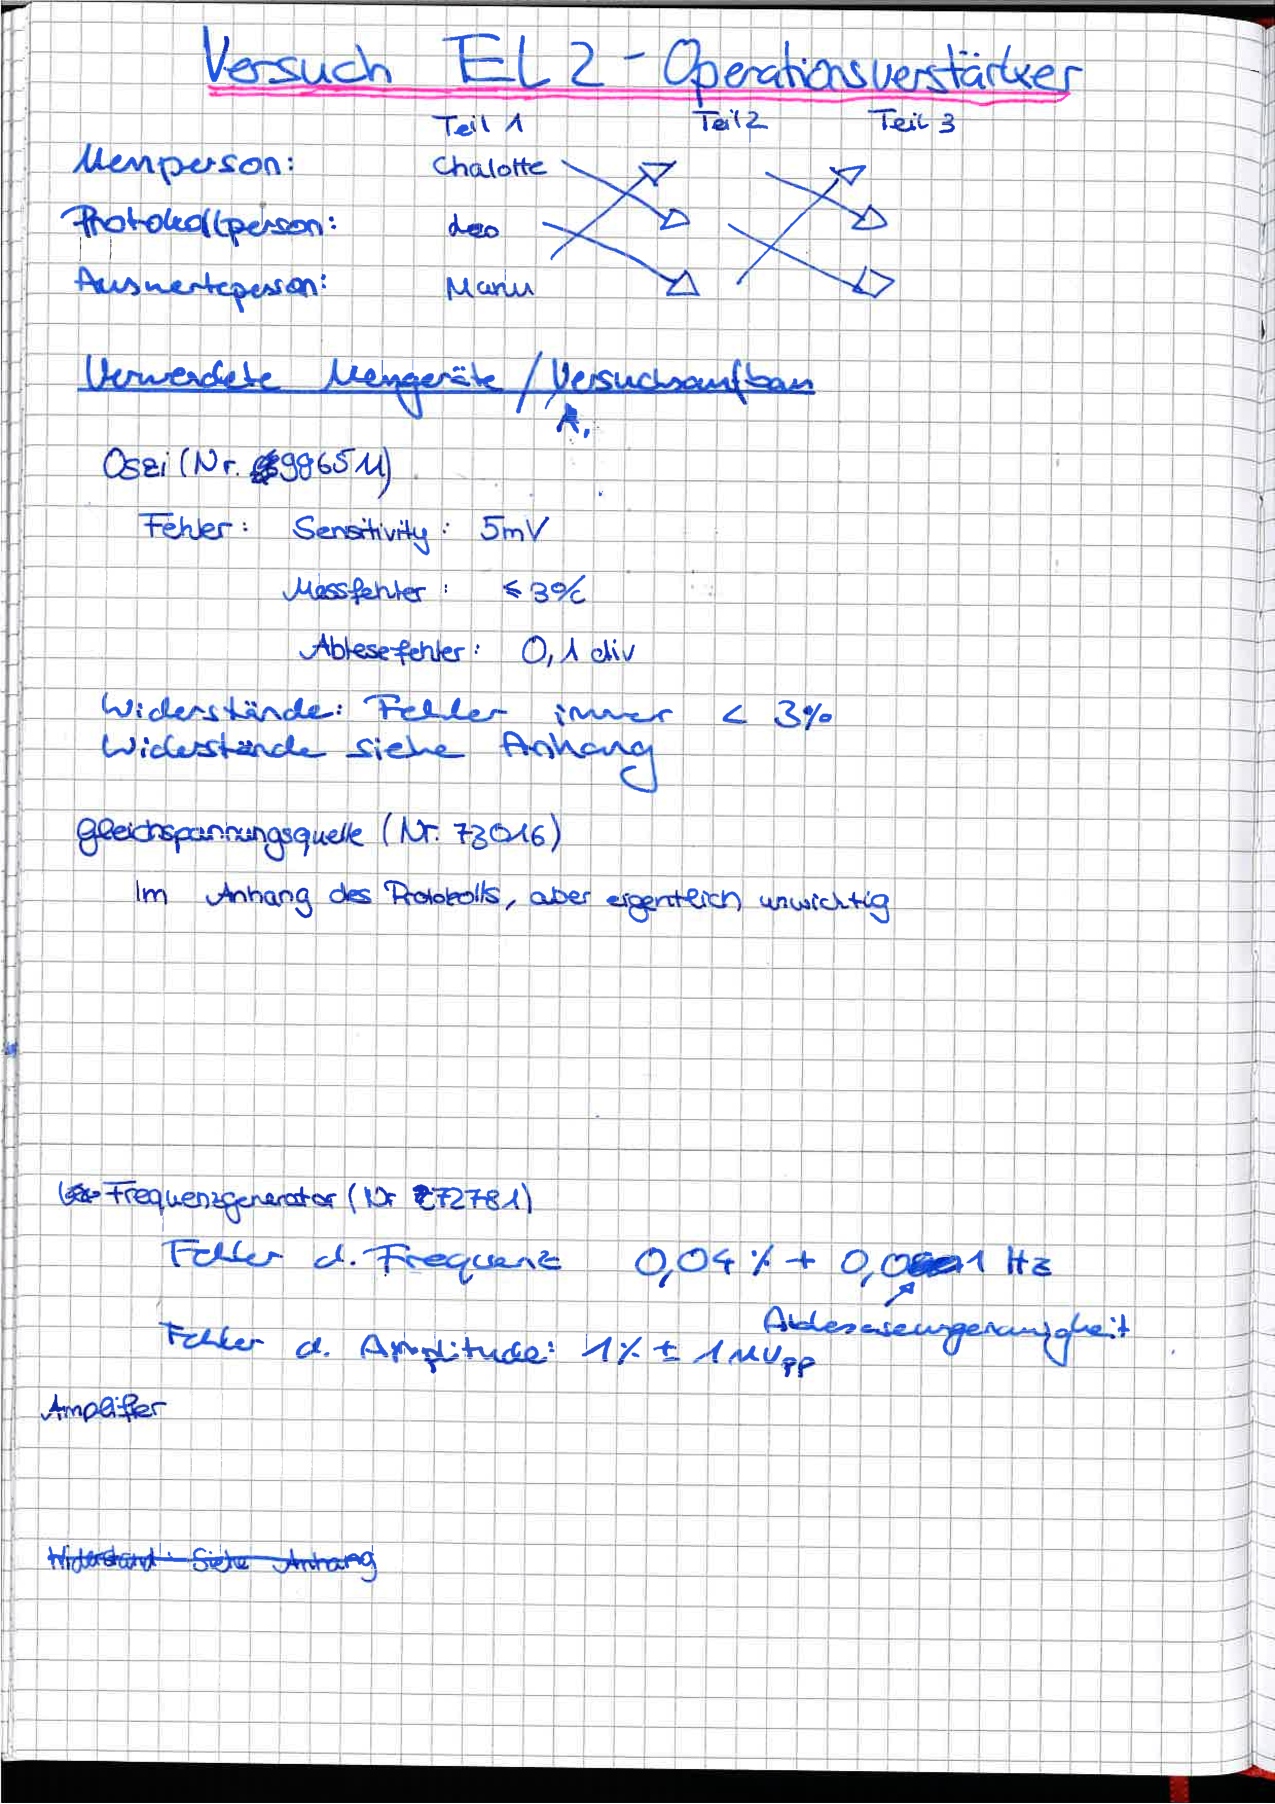
\includepdf[pages = -, landscape = false, nup = 1x1, scale = \skalierung , pagecommand={}]{30-ProtokollEL2.pdf}
\section*{Zusatz}

\section*{Umkehrintegrator}
\begin{center}
    \captionof*{figure}{10 Hz}
    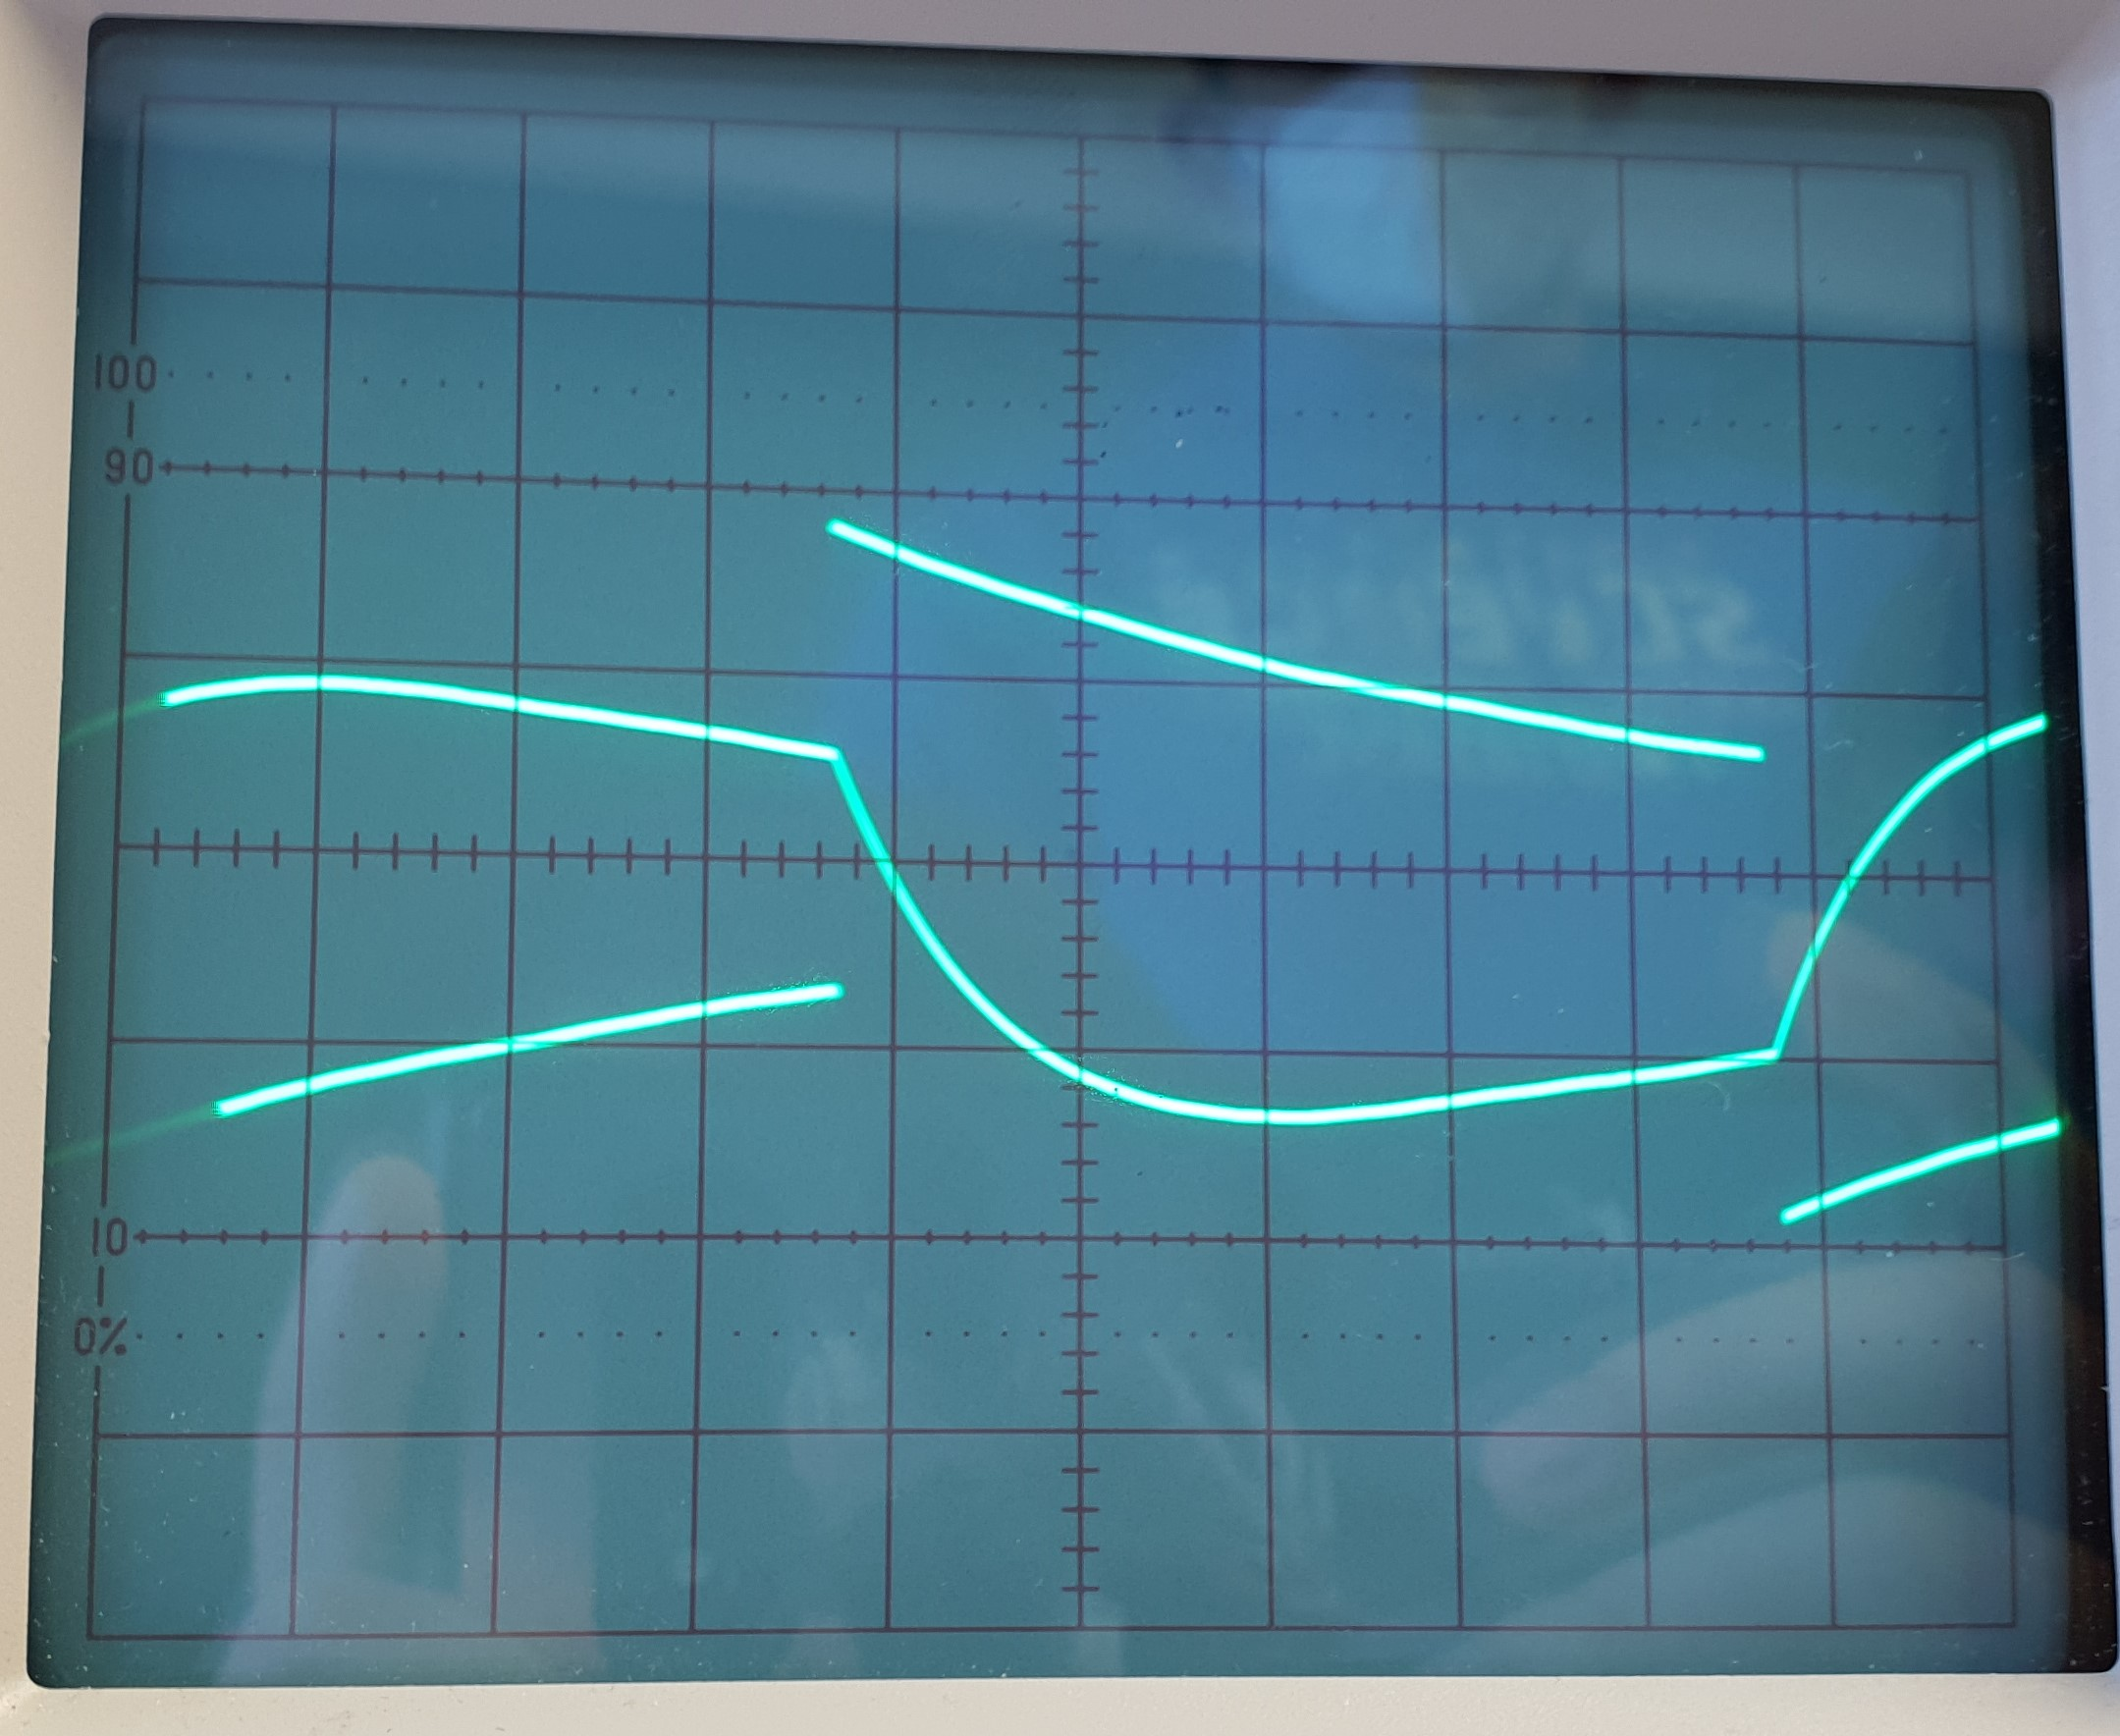
\includegraphics[width = 6.5cm]{42-10Hz.jpg}
    \captionof*{figure}{100 Hz}
    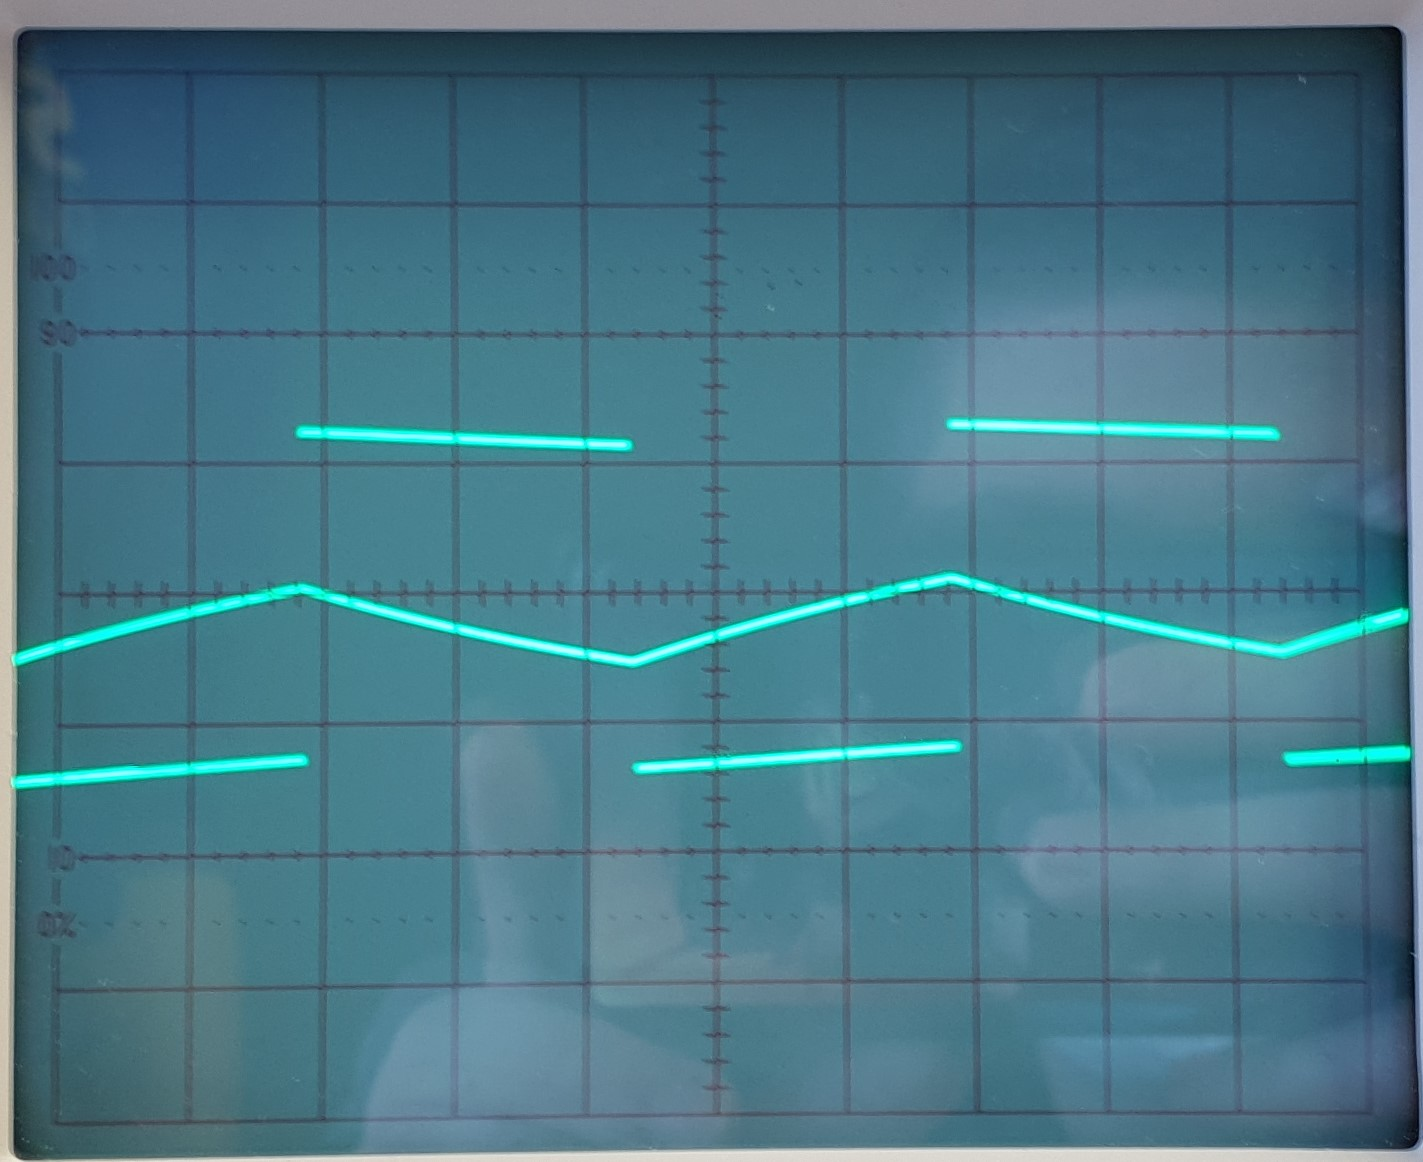
\includegraphics[width = 6.5cm]{42-100Hz.jpg}
    \captionof*{figure}{1000 Hz}
    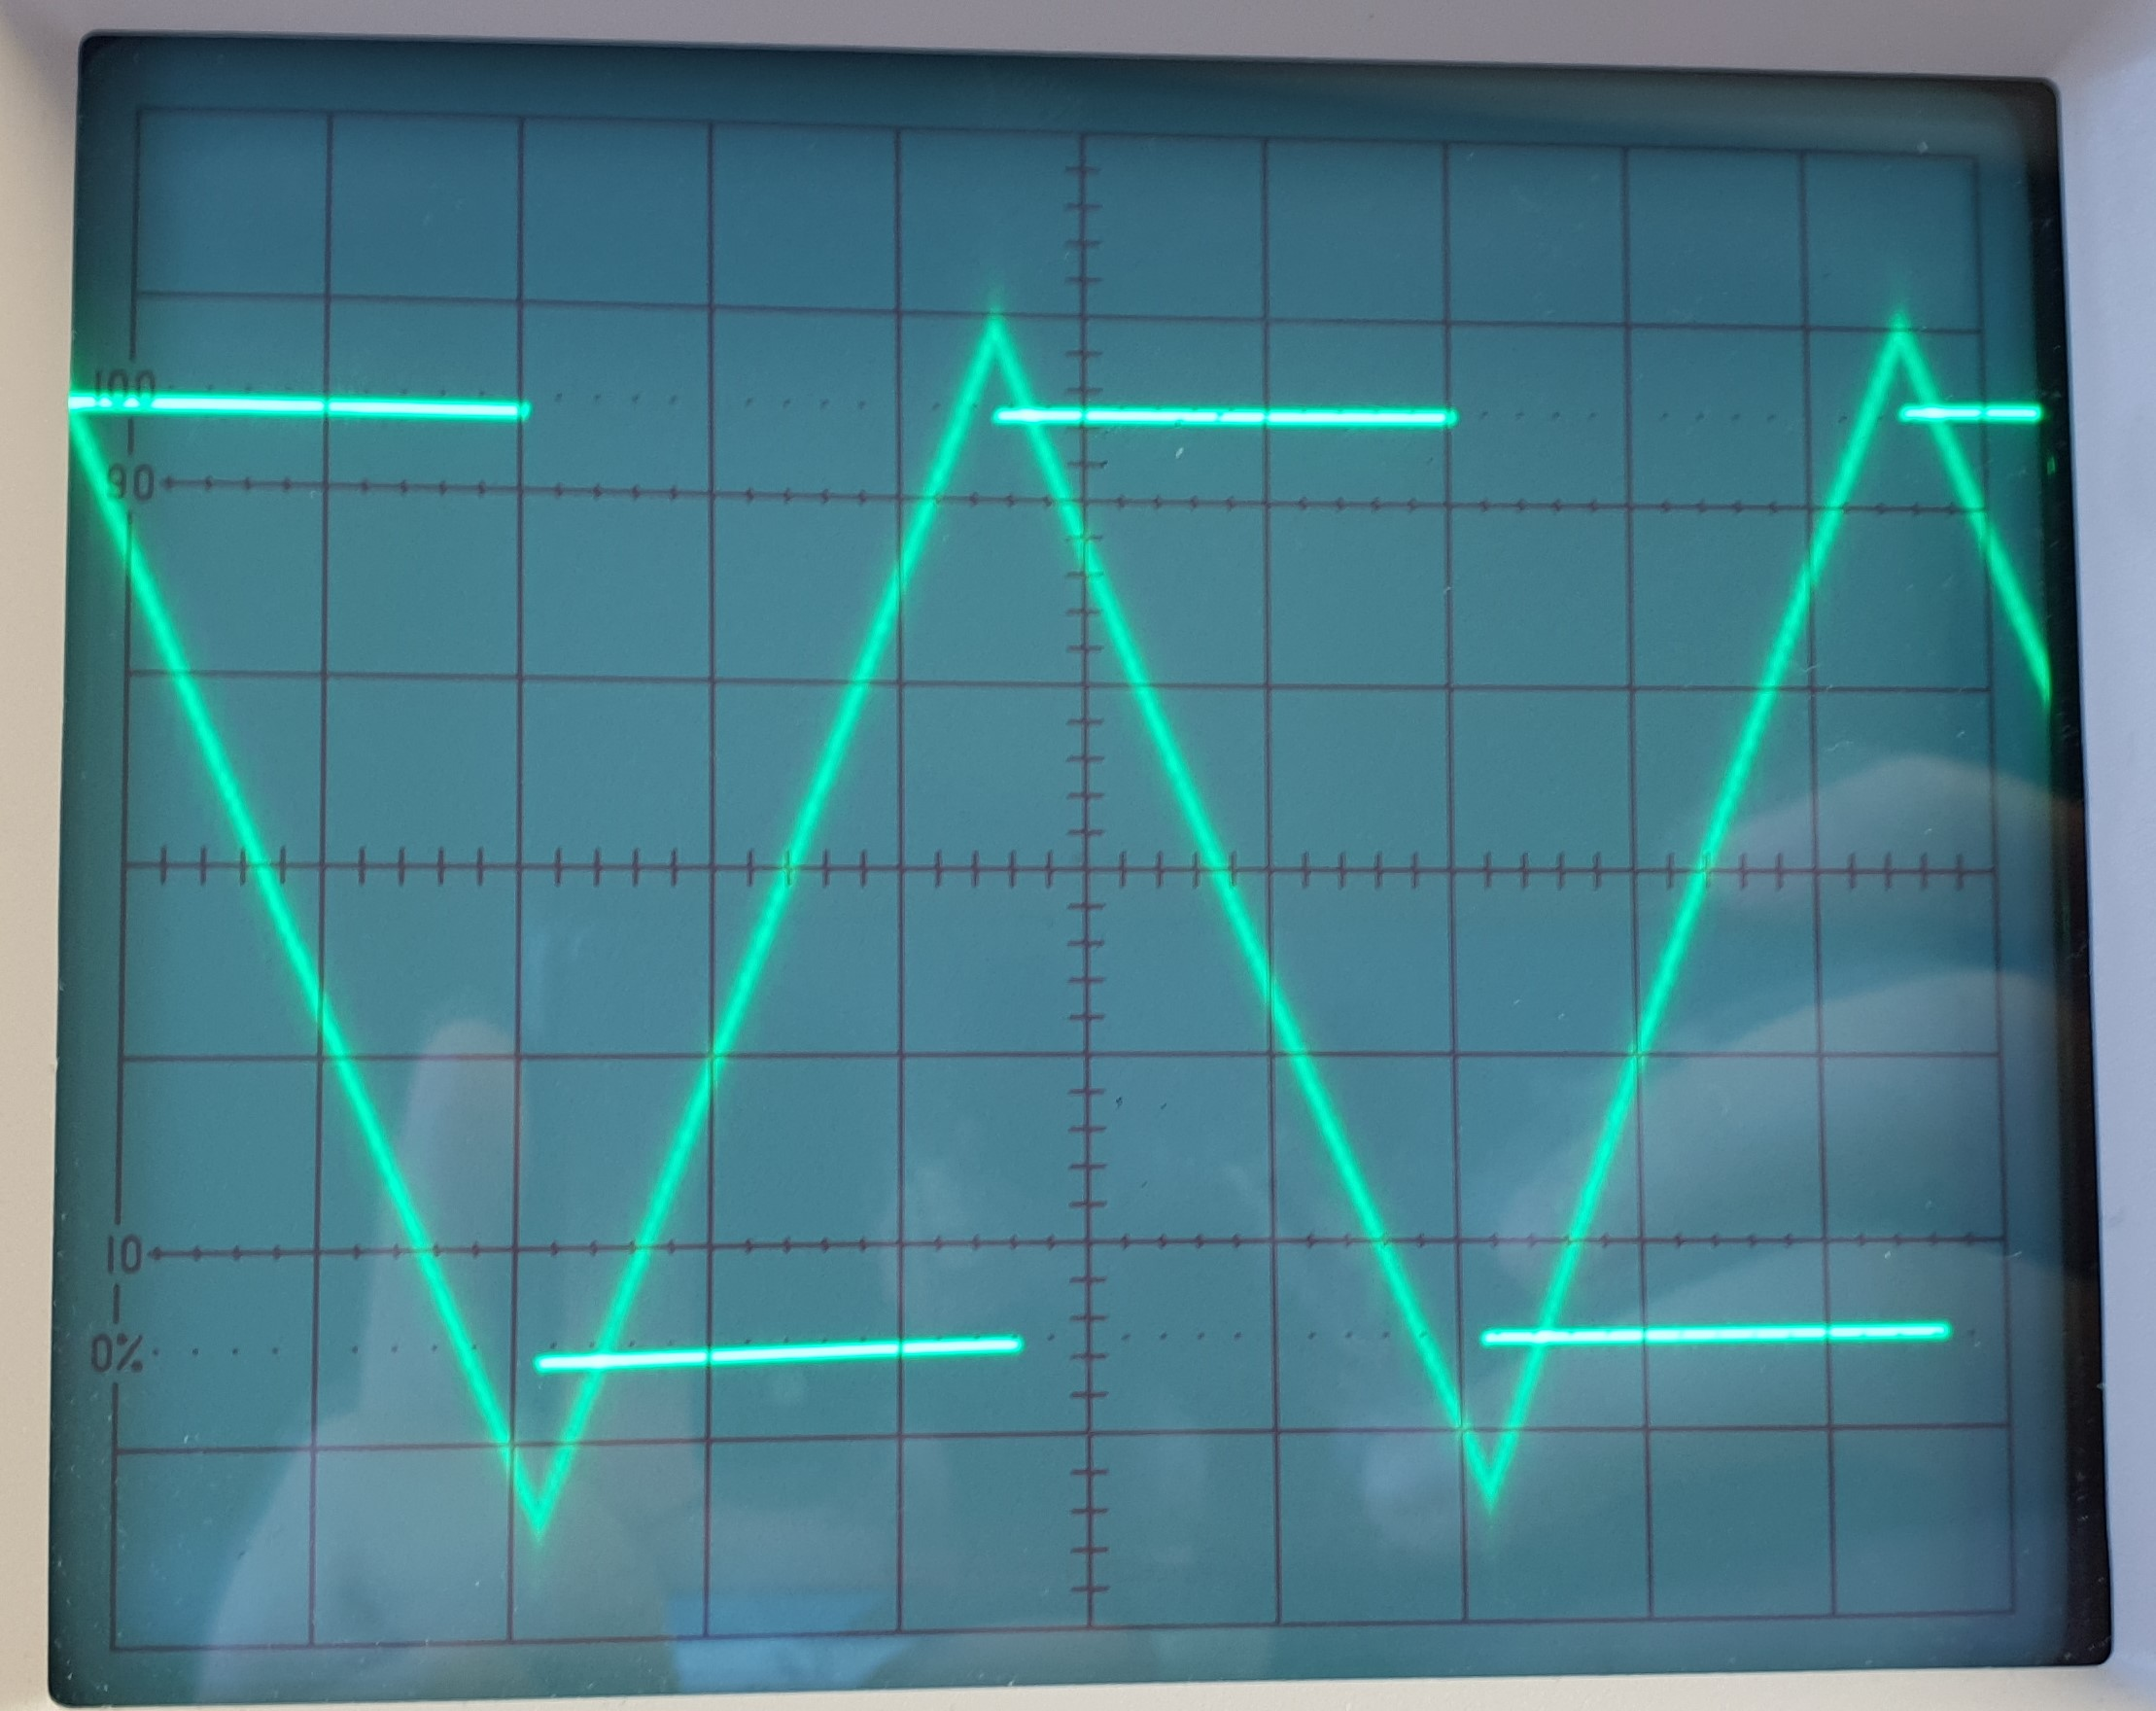
\includegraphics[width = 6.5cm]{42-1000Hz.jpg}
\end{center}

\section*{Umkehrdifferenzierer}
\begin{center}
    \captionof*{figure}{OPV mit $R_2, C_1$ bei $f=1~\text{kHz}$}
    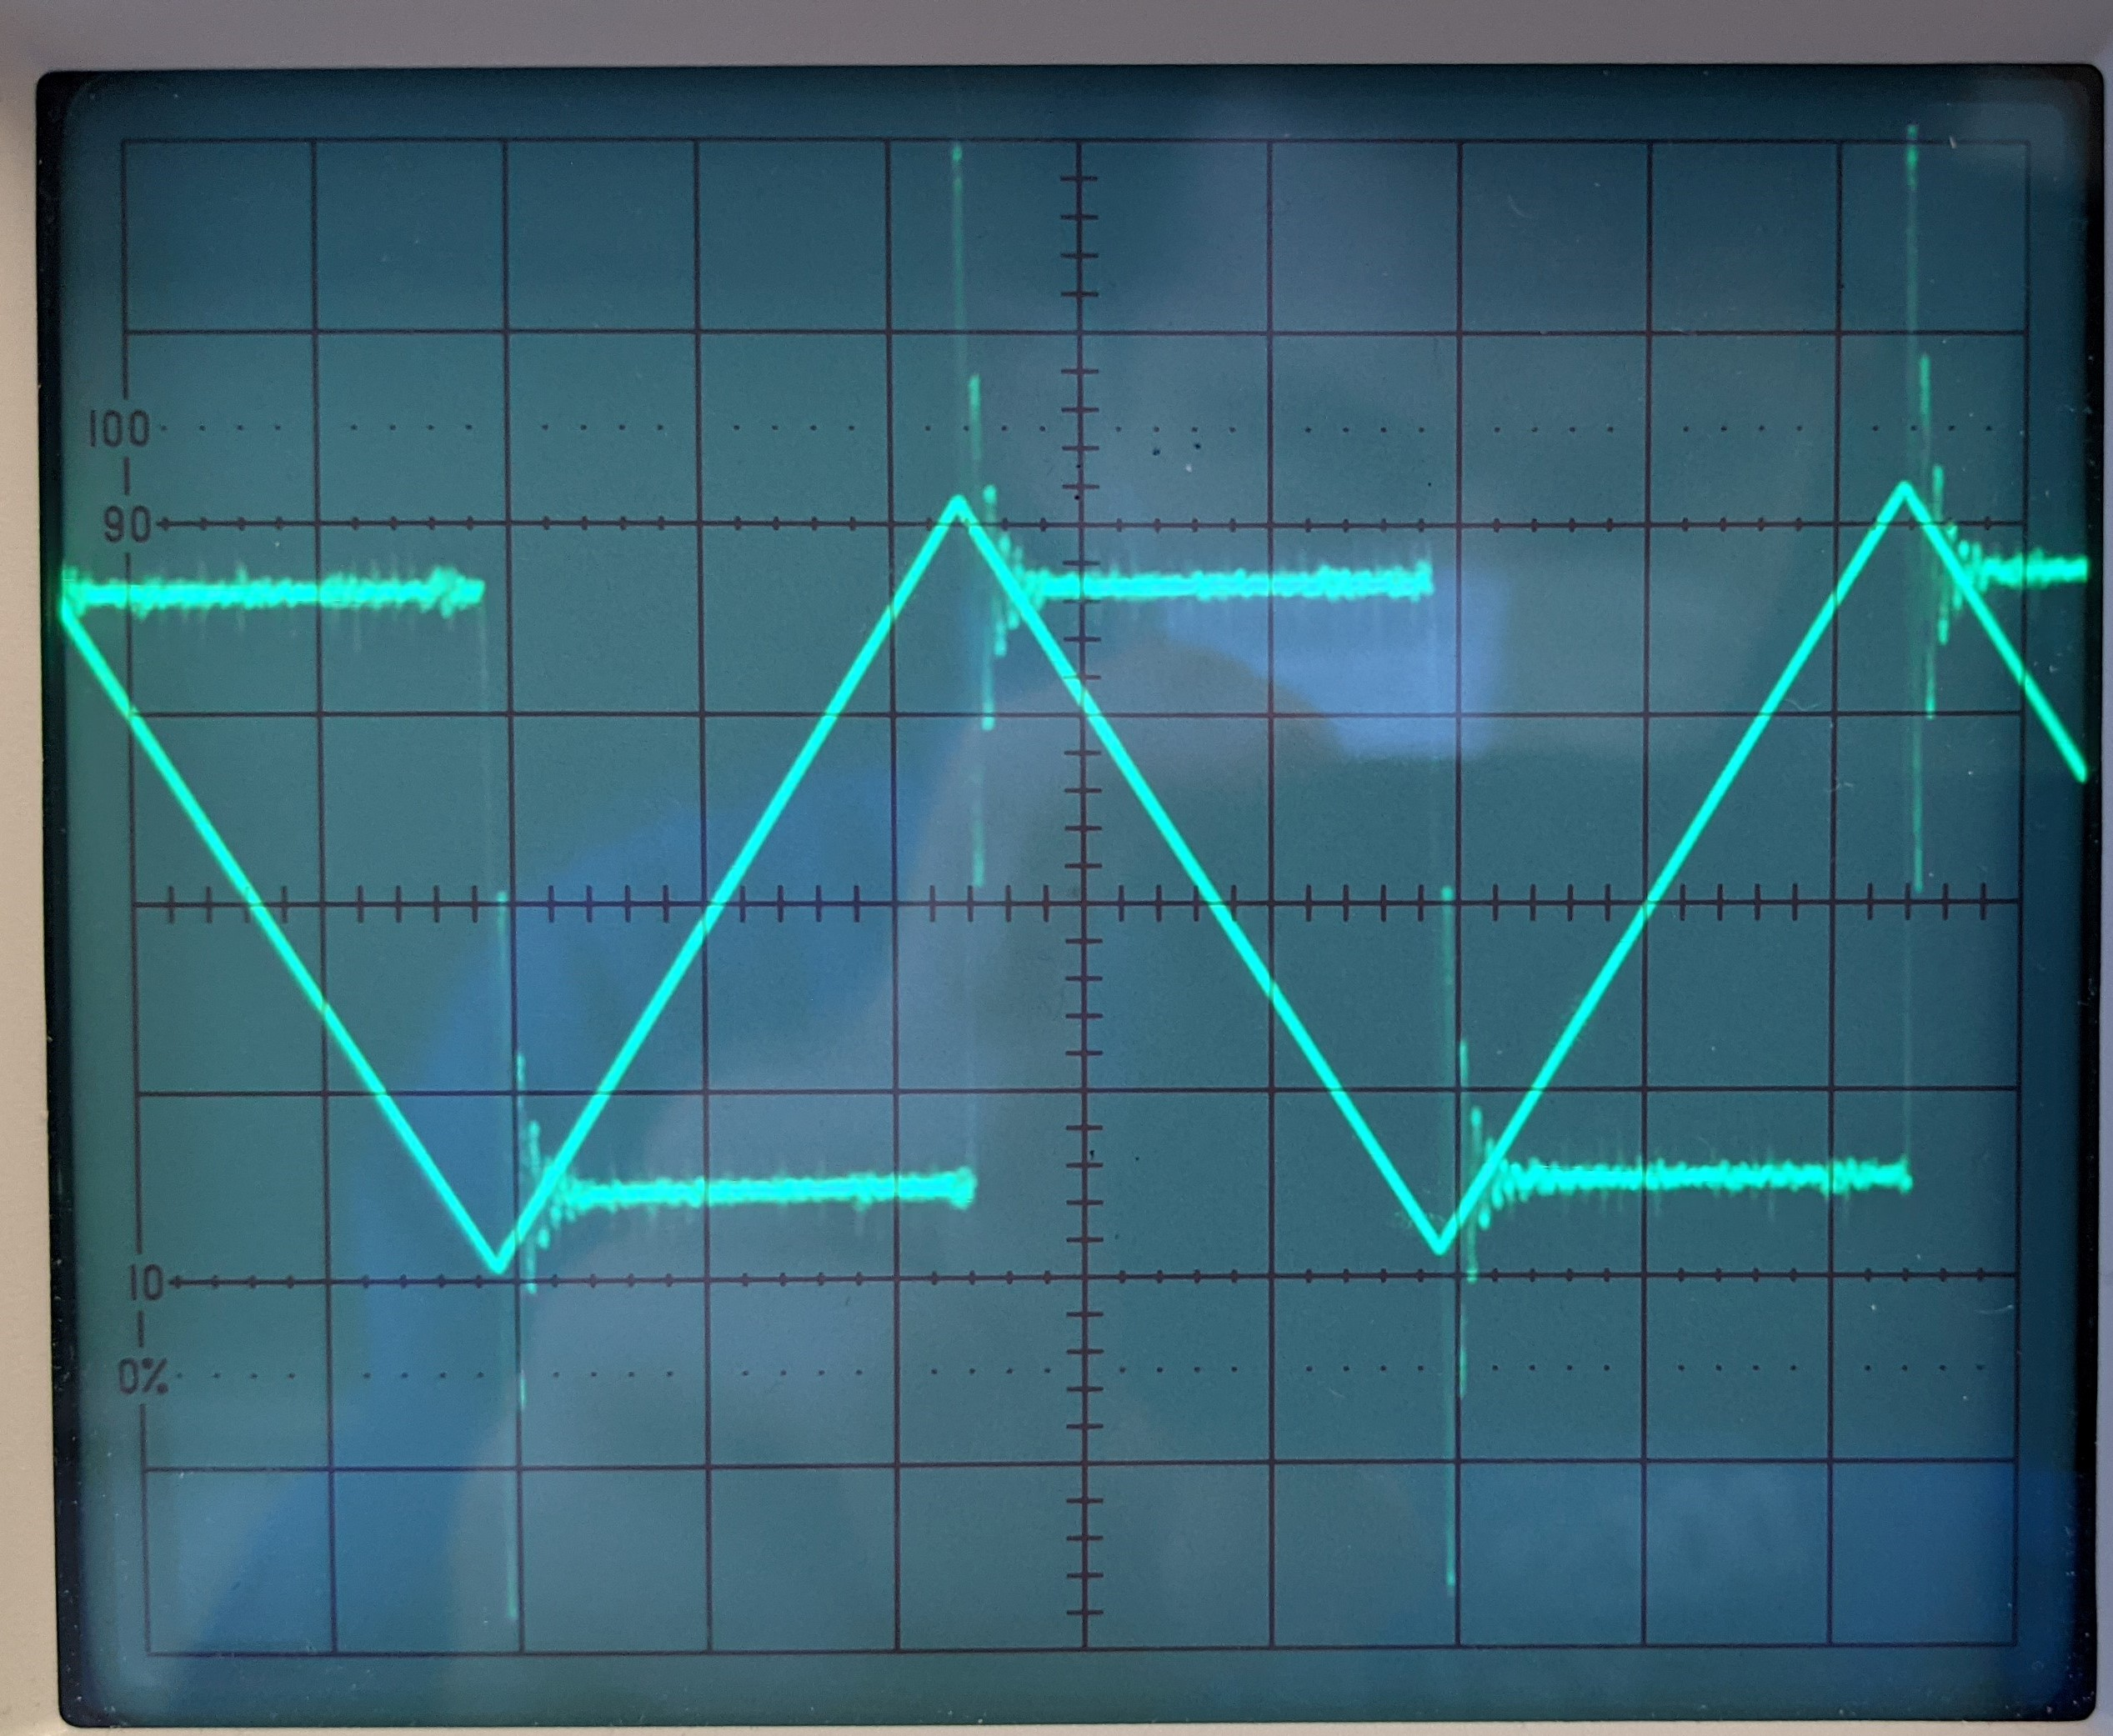
\includegraphics[width = 8cm]{43-diffSchwingung.jpg}
    \captionof*{figure}{OPV mit $R_1, R_2, C_1, C_2$ bei $f=1~\text{kHz}$}
    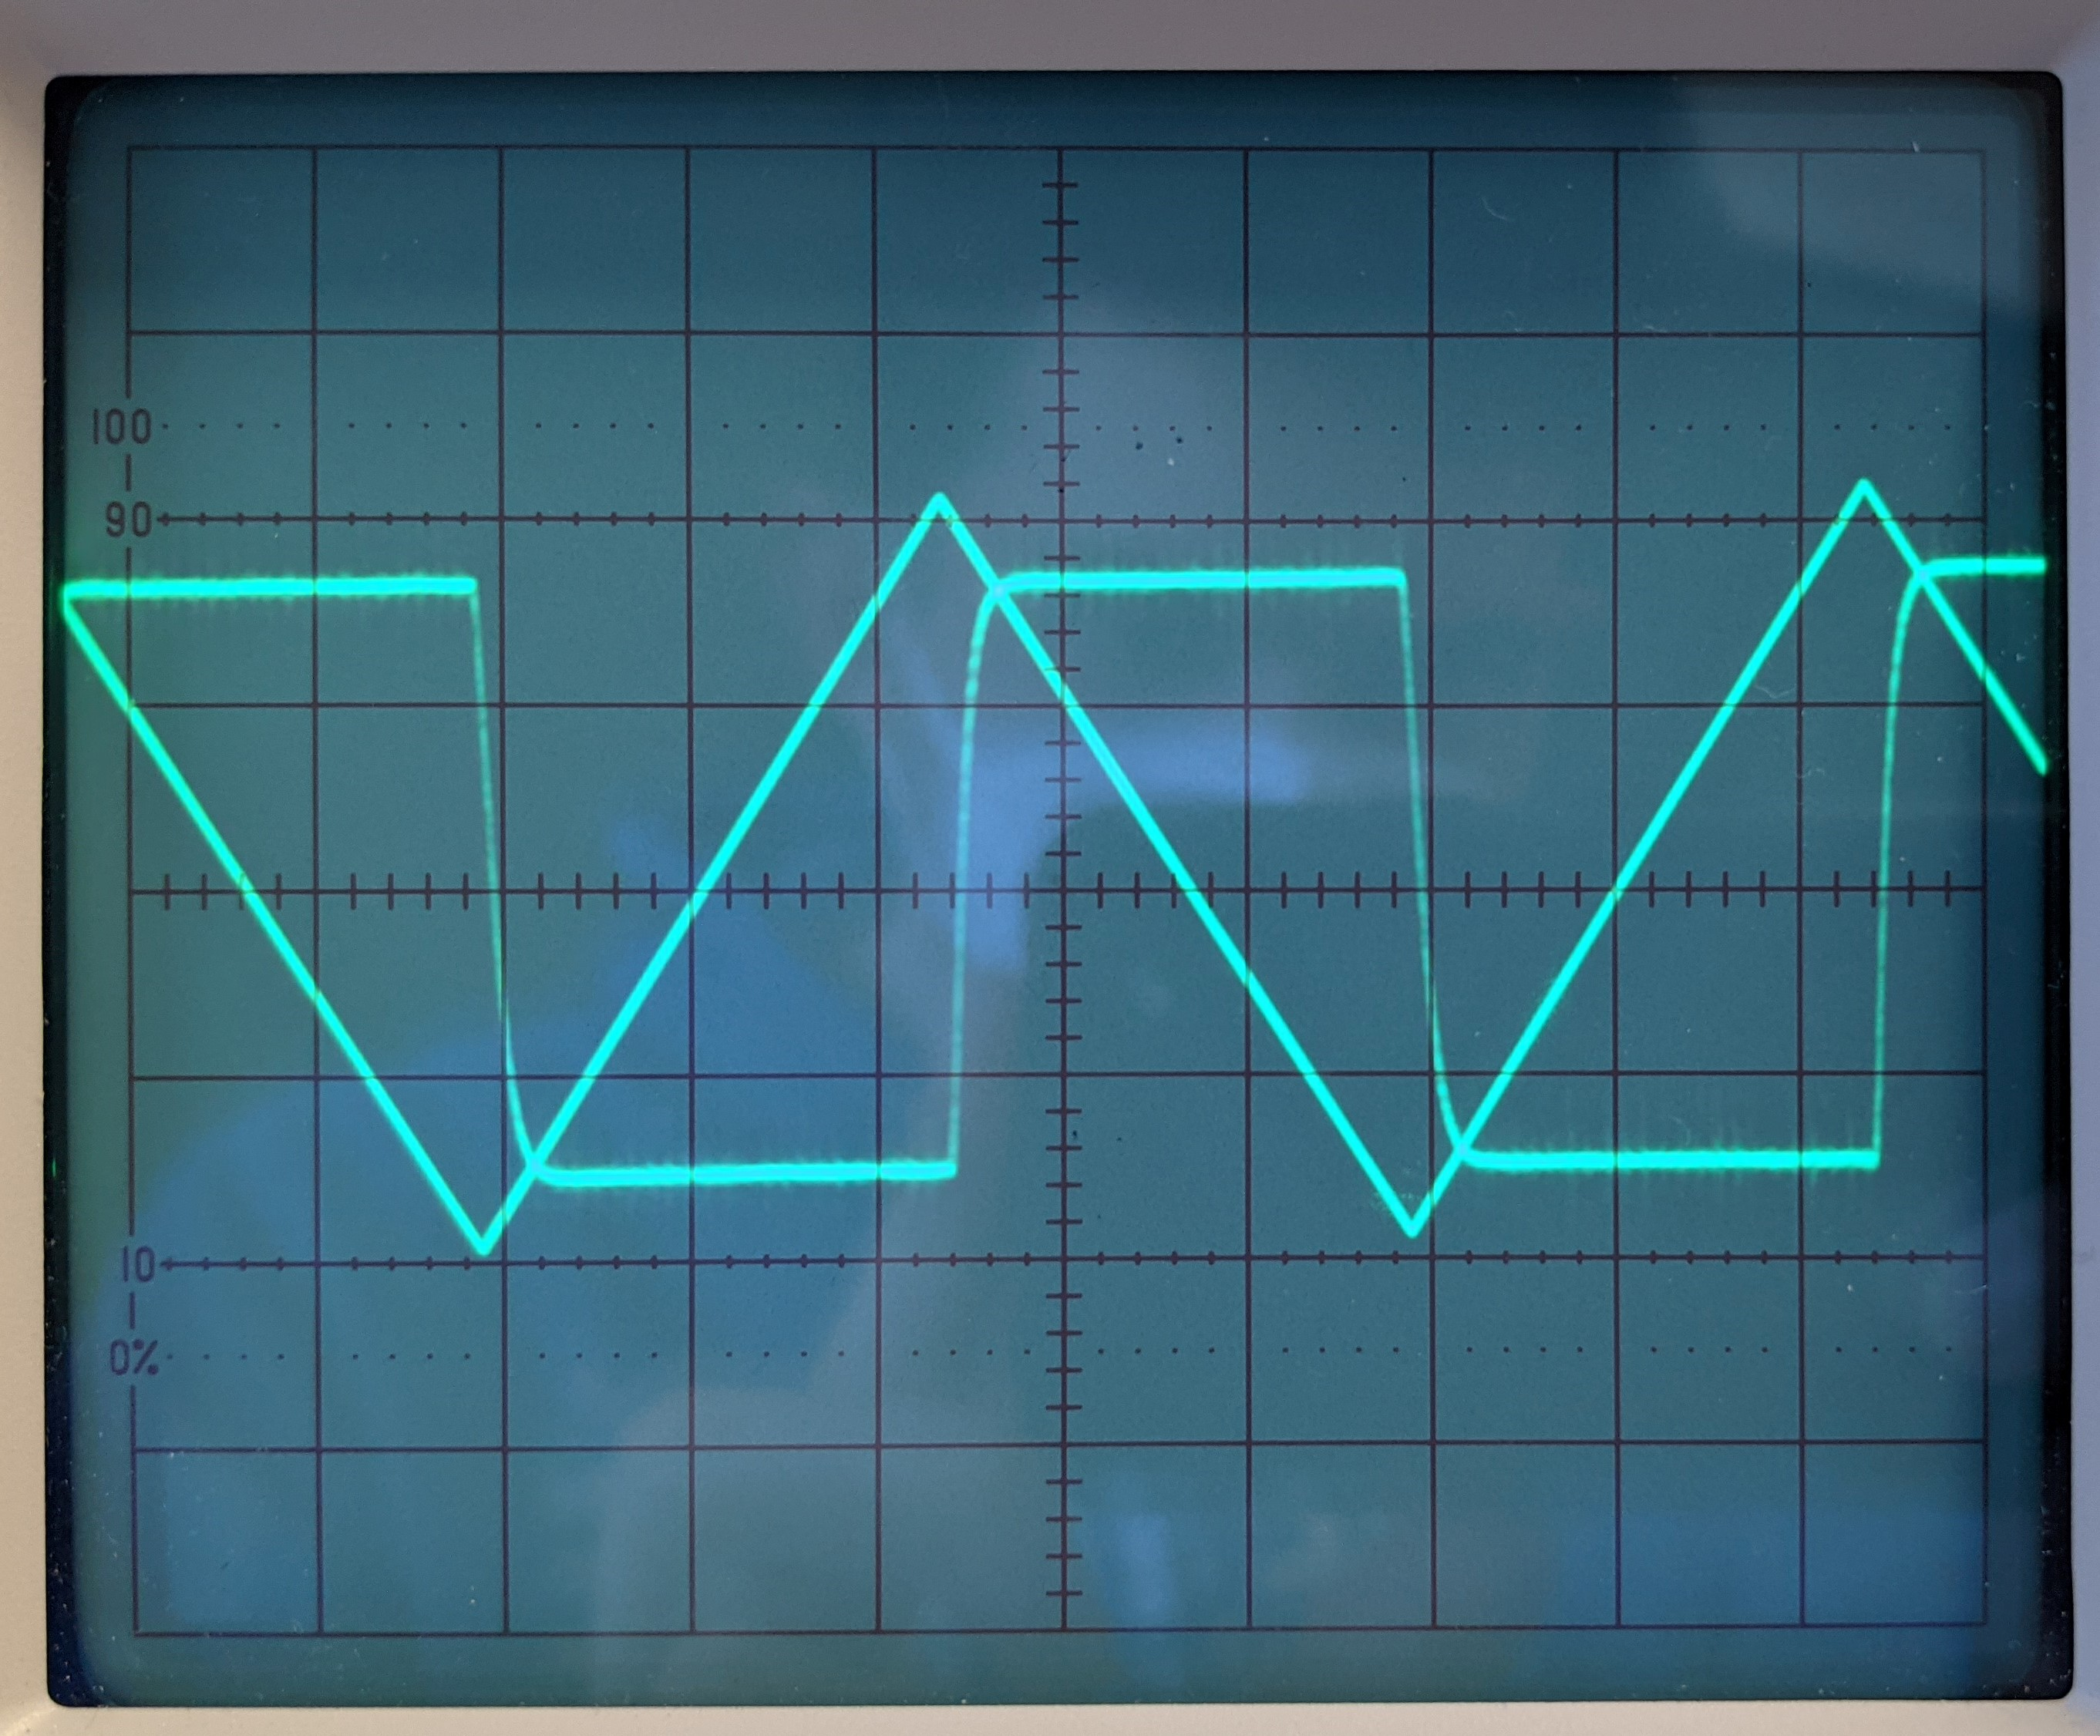
\includegraphics[width = 8cm]{43-diffStabil.jpg}
\end{center}
\newpage
\section*{Widerstände}
\begin{center}
    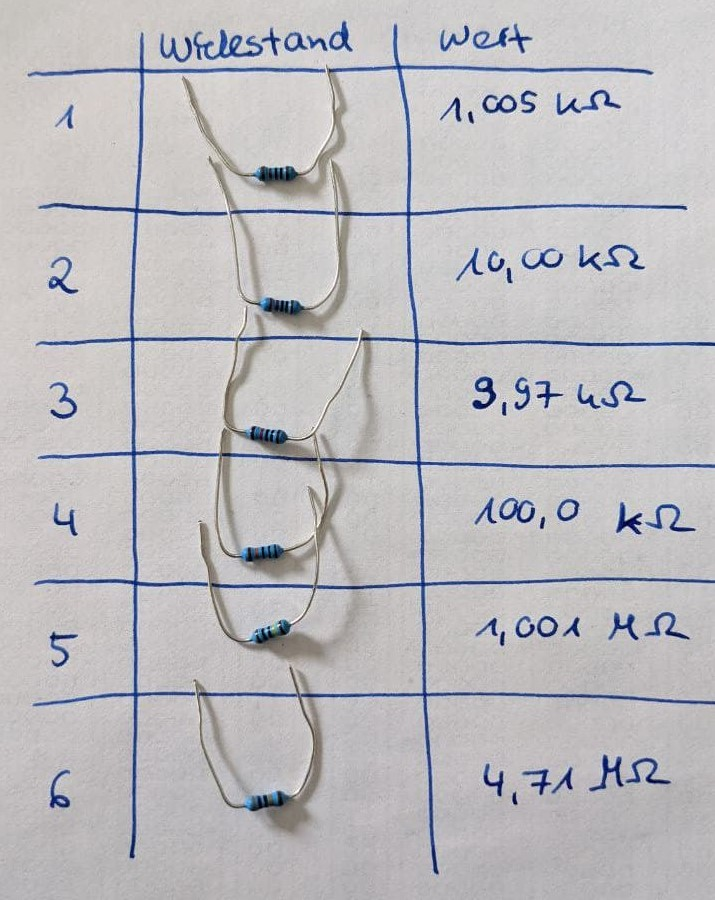
\includegraphics[scale = 0.5]{widerstaende.jpg}
\end{center}

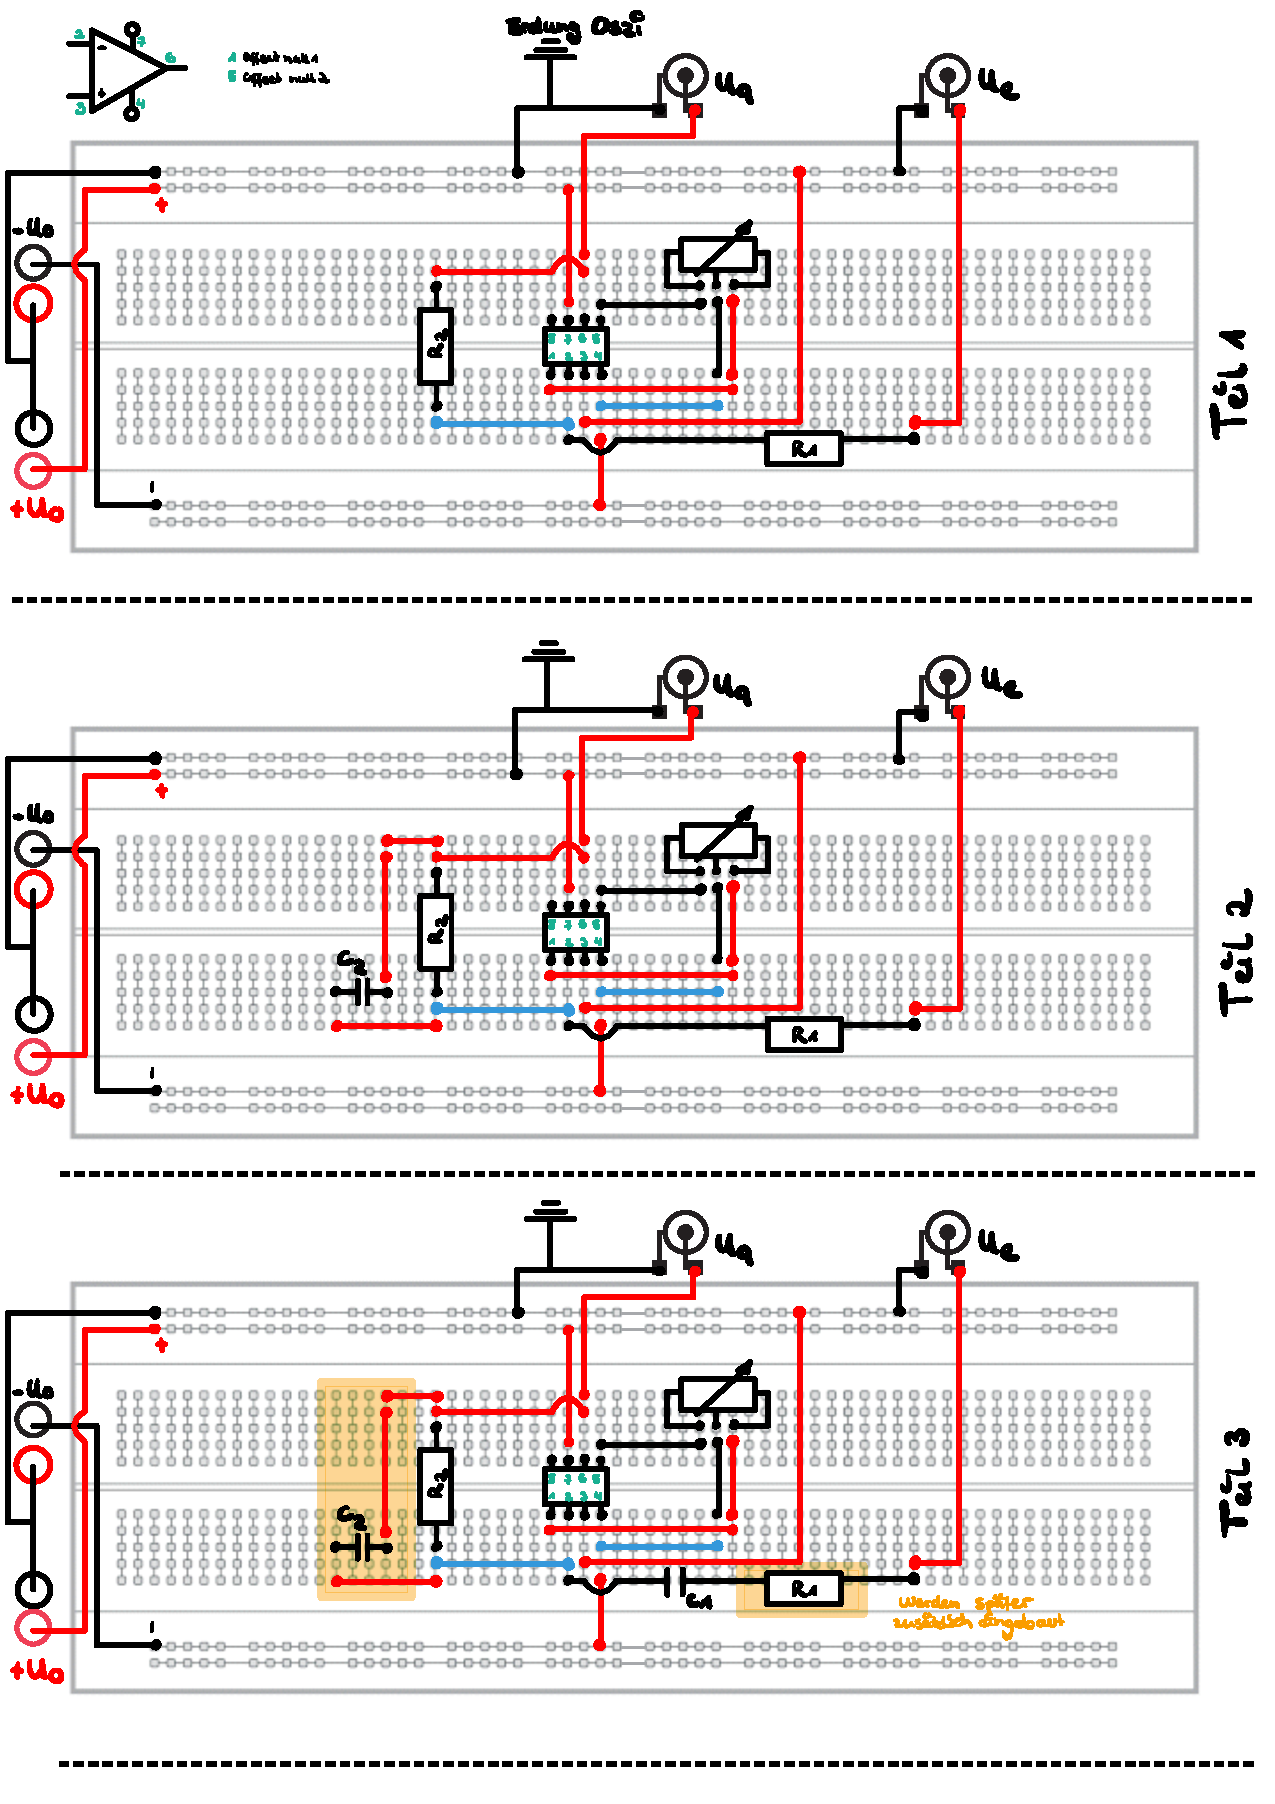
\includepdf[pages = 1, landscape = false, nup = 1x1, scale = \skalierung , pagecommand={\section*{Steckbretter}}]{30-SteckbretterEL2.pdf}